%!TEX = xelatex
\documentclass[a4paper]{article}
\usepackage[margin=1in]{geometry}
\usepackage{graphicx}
\usepackage{amsmath}
\usepackage{amssymb}
\usepackage{xcolor}
    \newcommand{\todo}[1]{\textcolor{red}{[ #1 ]}}
    \newcommand{\instruction}[1]{\textcolor{orange}{#1}}
    % \renewcommand{\todo}[1]{} % Uncomment to hide todos.
    % \renewcommand{\instruction}[1]{} % Uncomment to hide instructions.

\newcommand{\hidden}[1]{}

\usepackage{biblatex}
    \addbibresource{references.bib}

\usepackage[colorlinks=false]{hyperref}

\title{STATS 402 - Interdisciplinary Data Analysis\\
    Resource-Constrained Deep Reinforcement Learning for Battlesnake\\
    Milestone Report: Stage 3
}
\author{Steven Hé (Sīchàng)\\
    sichang.he@dukekunshan.edu.cn
}

\begin{document}
\maketitle

\subparagraph{Abstract}

Battlesnake~\cite{battlesnake}.

\instruction{
    There are no specific requirements for the stage 3 report since the progress
    may vary among different groups. Generally,
    there are four parts you need to cover in your report.
}

\section{Current Status}

\todo{
    For example, the detailed techniques you adopted to conduct the project.
    Has your group made any technical route adjustments?
    This part is essential for the groups whose actual adopted method is
    different from their milestone report 1 and report 2.
    You need to explain the reason for the change.
}

% TODO: Cite VGG and PyTorch.
We constructed convolutional neural network (CNN) layers for feature extraction,
referencing the VGG16 model.
Our feature layers consist of the first 7 convolutional layers,
the first 3 max-pooling layers, and the adaptive average layer in VGG16,
incrementally compressing the input feature matrices from $\mathbb R^{9\times
            21\times 21}$ to $\mathbb R^{256\times 2\times 2}$.
The features are then flattened and fed into 3-layer MLPs with hidden layer
widths 256 for either policy or value networks.

We constructed a shallower and thinner model than the VGG16 model primarily for
two reasons: our feature matrices are smaller,
and our compute resources are limited.
We only used the first 3 max-pooling layers because our feature matrices have
width 21 instead of the 224 in VGG16. That is,
after all 5 max-pooling layers with kernel size 2 in VGG16,
the feature matrices would be compressed from width 224 to 7; in comparison,
our feature matrices are compressed from width 21 to 2 after 3 similar
max-pooling layers.
Additionally, we believe that the game board of Battlesnake is simple enough,
that $256\times 2\times 2=1024$ numbers are sufficient to extract the features,
and MLP layers with width 256 are sufficient to learn these smaller features.

After initial testing, the VGG-like model performed poorly,
therefore we added a residual layer to it.
Our reasoning is the CNN layers may lose the positional information,
e.g., the snake's head is always at the center of the feature matrices;
also, the network's larger depth might result in the vanishing gradient problem.
The residual is a 2-layer MLP with hidden layer of width 2048,
transforming the input features from $\mathbb R^{9\times 21\times 21}$ to
$\mathbb R^{1024}$ before adding them to the output of the CNN layers.

deeper MLP feature extractor with 4 hidden layers of width 1024 and a residual
layer.

small modified vision transformer (ViT) with patch size 7, 4 encoder layers,
4 heads, hidden size 256, and MLP size 512.

We realized the default entropy coefficient of 0 in the Stable Baselines3 implementation has been used

\section{Existing Results}

\todo{Demonstrate all the existing results you obtained.}

The VGG-like model took around 2000 seconds to train for $16^4$ steps using all
CPU cores on the aforementioned server,
about 10 times longer than the MLP model.

Although we worried about the size of the model impacting the inference speed,
inference only took less than 1.0 millisecond and 600\,MiB of RAM on the default
Duke VM. Therefore,
we believe inference speed is not a bottleneck even on compute-constrained
environments,
but the size of the model will become a bottleneck when RAM is limited.
As a conclusion,
larger and more resource-intensive models like transformer are likely feasible,
with the training process being the major bottleneck.

The VGG-like model performed poorly, even after we added the residual layer,
and trained for $51 \times 16^4$ steps. During manual inspection,
the model cannot even consistently avoid walls,
which we consider a rudimentary learning task.
We suspect that the convolutional layers loose the positional information,
which is particularly significant in our case because our feature extraction
steps center the snake's head in the feature matrices. However,
another great possibility is the model requires much more training steps due to
its significantly larger size.

% TODO: Discuss how many steps are needed, referring to the Medium article.

If trained without any entropy bonus,
larger models have a tendency to instruct the snake to spin in a circle.
The deeper MLP model converged to go in a tight circle by keep turning left,
after less than $3\times 16^4$ steps, and all future models remained so.
Similarly,
it is observed that the ViT model stays in a tight left-turn circle when the
snake gets into certain positions,
after the model is trained for $72\times 16^4$ steps.
Convergence to spinning happens because of lack of exploration.
At the beginning of training,
the model cannot avoid walls or other snakes consistently,
therefore spinning produces better results than moving around because it avoids
running into walls or snakes, despite making the snake starve to death.
Since there is no entropy bonus,
the model never has a chance to explore better moves,
and eventually converges to spinning.

\begin{figure}
    \centering
    % TODO: \includegraphics[width=0.4\linewidth]{deep_mlp_spin_render.png}\quad
    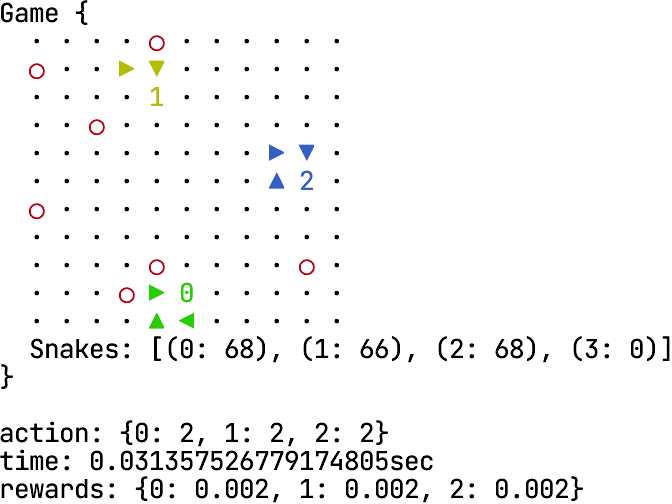
\includegraphics[width=0.4\linewidth]{vit_spin_render.png}
    \caption{TODO
    }
    \label{fig:render}
\end{figure}

\section{Final Report Plan}

\todo{The plan for finalizing your final report.}

\section{Notes}

\subsection{Training Customization}

We directly customized the training loop in Stable
Baselines3~\cite{raffin2024stable}
to simplify the logic and prepare for the implementation to train the agent
against older versions of itself for 20\% of the time.
Because Battlesnake is a multi-player simultaneous-move game,
and Stable Baselines3 only supports single-agent environments,
previously, we created our environment
following the Pettingzoo~\cite{terry2021pettingzoo} parallel environment API,
and used SuperSuit~\cite{SuperSuit} to wrap it.

However, using SuperSuit for wrapping introduces two major downsides. First,
complexity is massively increased,
as SuperSuit requires multiple layers of wrappers.
This obstructs the understanding of the training process and hinders any
modifications to it, such as the old-version self-training. Second,
SuperSuit produces empty observations and zero rewards for dead agents,
so they appear alive,
and the environment appears to be a Stable Baselines3 vectorized environment.
These useless padding not only wastes computation during training,
but raises uncertainty.
Since dead agents' actions are counted into the number of steps the model has
trained, it is unclear how many steps the model has actually trained.
Additionally, it is unclear how the padding affects the training.

We modified and overrode the training methods on Stable Baselines3's PPO
implementation. Our implementation tracks each agent's statistics separately,
and only pushes them to calculate the returns and advantages when the agent
dies. We also correctly count the number of steps the model has trained,
by summing the number of steps each alive agent moves.
Although our implementation is not vectorized,
it still uses all available CPU cores on our server with dual EPYC 7763 64-Core
processors. Training for $16^5$ steps took 3777 seconds,
longer than the 3060 seconds the previous implementation took. However,
we note that the previous training was counting padding steps,
meaning that the new implementation has effectively trained more steps.

\printbibliography

\end{document}
